\documentclass[tikz]{standalone}
\usepackage{amsmath}
\usepackage{tikz}

\begin{document}

\begin{figure}[H]
\begin{center}
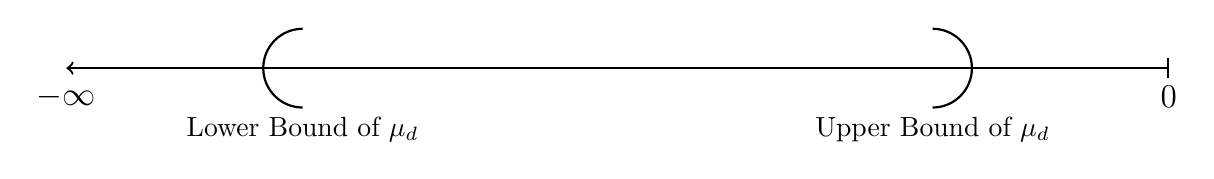
\begin{tikzpicture}
  \draw[<-|, thick] (-7,0) -- (7,0);
  \draw[thick] (-4,-0.5) arc (270:90:0.5);
  \node[below] at (-4,-0.5) {Lower Bound of $\mu_d$};
  \draw[thick] (4,0.5) arc (90:-90:0.5);
  \node[below] at (4,-0.5) {Upper Bound of $\mu_d$};
  \node[below] at (-7, -0.1) {\large$-\infty$};
  \node[below] at (7, -0.1) {\large$0$};
\end{tikzpicture}
\end{center}
\caption{Visualization of the case when $\bar{M}_1 < \bar{M}_2$}
\end{figure}

\end{document}